\section{Methodology}
Given an HSI cube $\mathbf{X}\in\mathbb{R}^{H\times W\times B}$ and sparse labels $\mathbf{Y}$, the proposed method extracts a local patch and a center spectrum for each labeled pixel. The spectral dimension can be reduced by principal component analysis (PCA) to suppress redundancy and improve training efficiency. The reduced cube is denoted as $\tilde{\mathbf{X}}\in\mathbb{R}^{H\times W\times C}$, where $C\leq B$.

For a labeled pixel at position $(i,j)$, the input consists of the center spectrum $\mathbf{s}_{ij}\in\mathbb{R}^{C}$ and a spatial patch $\mathbf{P}_{ij}\in\mathbb{R}^{C\times p\times p}$. DR-GSMamba processes this input through three branches: a spectral state-space encoder, a spatial convolutional stem, and a patch graph encoder. Fig.~\ref{fig:architecture} gives an overview of the framework.

\begin{figure*}[t]
\centering
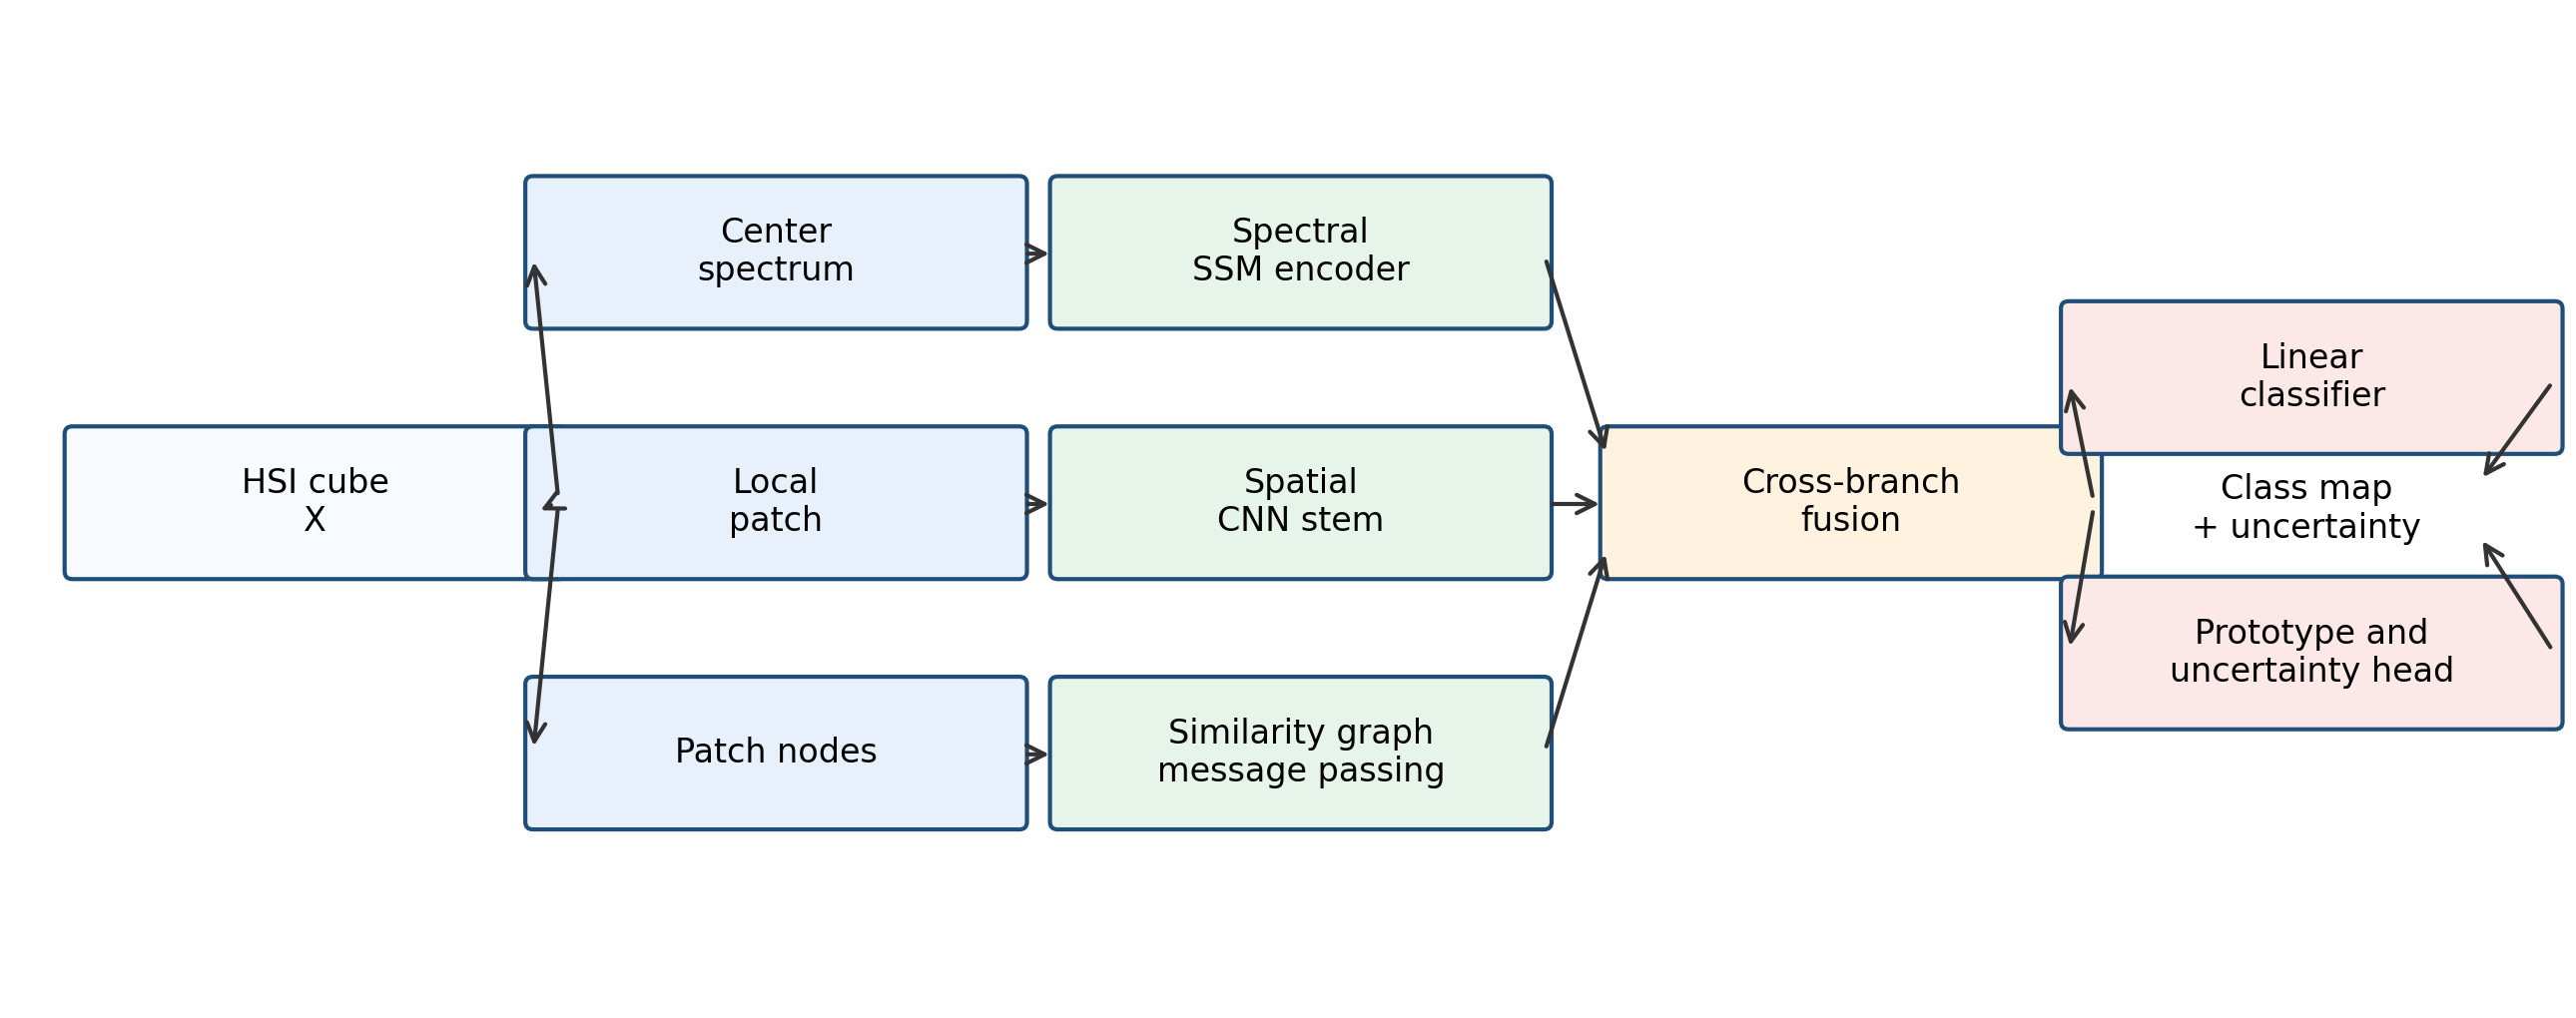
\includegraphics[width=0.95\textwidth]{figures/dr_gsmamba_architecture.png}
\caption{Overall structure of DR-GSMamba. The center spectrum is encoded by a spectral state-space branch, the local patch is processed by a spatial CNN stem, and patch nodes are aggregated through graph message passing. The fused feature is classified by linear and prototype heads, producing class predictions and uncertainty scores.}
\label{fig:architecture}
\end{figure*}

\subsection{Spectral State-Space Encoder}
The center spectrum is treated as a one-dimensional ordered sequence. Each scalar band value is projected into a hidden feature space. The sequence is then processed by stacked state-space style blocks. Each block contains layer normalization, gated projection, depthwise sequence mixing, and residual projection. This design follows the spirit of selective state-space modeling while avoiding an external CUDA dependency, making the implementation easy to reproduce.

Let $\mathbf{Z}^{(0)}\in\mathbb{R}^{C\times d}$ be the embedded spectral sequence. For the $l$-th block, the update is written as
\begin{equation}
\mathbf{Z}^{(l+1)}=\mathbf{Z}^{(l)}+\phi_{\theta}\left(\mathrm{LN}(\mathbf{Z}^{(l)})\right),
\end{equation}
where $\phi_{\theta}(\cdot)$ denotes gated depthwise sequence mixing. The final spectral representation $\mathbf{f}_{spec}$ is obtained by global average pooling over the sequence dimension.

\subsection{Patch Graph Reasoning}
Spatial features are extracted from $\mathbf{P}_{ij}$ using a compact convolutional stem. The resulting feature map is reshaped into $N=p^2$ patch nodes. Each node corresponds to one spatial location inside the patch. To build a soft graph, node features are normalized and their pairwise similarities define an adjacency matrix:
\begin{equation}
\mathbf{A}=\mathrm{softmax}\left(\frac{\mathbf{Q}\mathbf{Q}^{T}}{\sqrt{d}}\right),
\end{equation}
where $\mathbf{Q}\in\mathbb{R}^{N\times d}$ contains normalized node features. Graph message passing is then performed as
\begin{equation}
\mathbf{H}^{(l+1)}=\mathrm{LN}\left(\mathbf{H}^{(l)}+\sigma(\mathbf{A}\mathbf{H}^{(l)}\mathbf{W}^{(l)})\right),
\end{equation}
where $\sigma(\cdot)$ is the GELU activation. The patch graph representation $\mathbf{f}_{graph}$ is obtained by averaging node features after message passing.

\subsection{Prototype and Uncertainty Head}
The spectral, spatial, and graph representations are concatenated and projected into a fused feature $\mathbf{f}$. A linear classifier predicts logits $\mathbf{o}_{lin}$, and a prototype head computes similarity logits $\mathbf{o}_{proto}$ using learnable class prototypes:
\begin{equation}
\mathbf{o}_{proto}=\tau \cdot \frac{\mathbf{f}}{\|\mathbf{f}\|_2}\frac{\mathbf{M}^{T}}{\|\mathbf{M}\|_2},
\end{equation}
where $\mathbf{M}$ is the prototype matrix and $\tau$ is a learnable scale. The final logits are $\mathbf{o}=\mathbf{o}_{lin}+\mathbf{o}_{proto}$. Prediction uncertainty is estimated from both predictive confidence and a learnable uncertainty head:
\begin{equation}
u=\frac{1}{2}\left(1-\max_k \mathrm{softmax}(\mathbf{o})_k\right)+\frac{1}{2}\tanh(\mathrm{softplus}(g_{\theta}(\mathbf{f}))).
\end{equation}
The learnable term is used during training to down-weight high-uncertainty samples while penalizing unbounded uncertainty.

\subsection{Robust Objective}
The training objective combines standard cross entropy, sample-level CVaR, class-level distributionally robust risk, prototype consistency, supervised prototype compactness, uncertainty-weighted cross entropy, and node-level graph smoothness:
\begin{equation}
\mathcal{L}=\mathcal{L}_{ce}+\lambda_1\mathcal{L}_{dro}+\lambda_2\mathcal{L}_{proto}+\lambda_3\mathcal{L}_{unc}+\lambda_4\mathcal{L}_{graph}.
\end{equation}
The robust term combines the largest per-sample losses and the largest class-wise risks within a mini-batch:
\begin{equation}
\mathcal{L}_{dro}=\frac{1}{2}\mathrm{CVaR}_{\alpha}(\{\ell_n\})+\frac{1}{2}\mathrm{CVaR}_{\alpha}(\{\bar{\ell}_c\}),
\end{equation}
where $\ell_n$ is the sample loss and $\bar{\ell}_c$ is the mean loss of class $c$ in the mini-batch. This gives the distributionally robust claim a concrete optimization target: difficult samples and high-risk classes both affect the gradient. Prototype consistency aligns the linear classifier with the prototype classifier, supervised prototype compactness pulls features toward their class prototypes, and graph smoothness regularizes node-level predictions over the learned patch graph.
